\chapter{Implementacija i korisničko sučelje}
		
		
		\section{Korištene tehnologije i alati}
		
			Komunikacija u timu realizirana je korištenjem platforme \underline{Whatsapp}\footnote{\url{https://www.whatsapp.com/}}. 
			Za izradu UML dijagrama korišten je alat \underline{Astah Professional}\footnote{\url{https://astah.net/products/astah-professional/}} i \underline{Visual Paradigm}\footnote{\url{https://online.visual-paradigm.com/}}, a kao sustav za upravljanje izvornim kodom \underline{Git}\footnote{\url{https://git-scm.com/}}. 
			Udaljeni repozitorij projekta je dostupan na web platformi \underline{GitLab}\footnote{\url{https://gitlab.com/}}.
			\par
			Kao razvojno okruženje korišten je \underline{IntelliJ IDEA}\footnote{\url{https://www.jetbrains.com/idea/}} - integrirano razvojno okruženje (IDE) tvrtke JetBrains i \underline{Eclipse}\footnote{\url{https://www.eclipse.org/ide/}}. 
            \par
            Aplikacija je napisana u \underline{Javi}\footnote{\url{https://www.java.com/en/}} koristeći ekosustav \underline{Java Spring}\footnote{\url{https://spring.io/}} za
            izradu backenda te \underline{React}\footnote{\url{https://reactjs.org/}} i jezik \underline{JavaScript}\footnote{\url{https://www.javascript.com/}} za izradu frontenda. 
            \par
            Baza podataka koju smo koristili je (\underline{PostgreSQL}\footnote{\url{https://www.postgresql.org/}}) i ona se nalazi na \underline{pgAdmin}\footnote{\url{https://www.pgadmin.org/}}.

            
            \vspace*{\fill}

			
			
			\eject 
		
	
		\section{Ispitivanje programskog rješenja}
			
Nakon što smo završili s izradom testirali smo rad aplikacije koristeći JUnit tehnologiju i Selenium WebDriver. Testovi su dali zadovoljavajuće rezultate te možemo zaključiti da smo uspjeli implementirati zadane funkcionalnosti.
			
			\subsection{Ispitivanje komponenti}
			
Za ispitivanje komponenti koristili smo JUnit tehnologiju. JUnit okvir je za testiranje komponenti sustava programiranog u Javi. Ispitali smo funkcionalnosti ažuriranja osobnih podataka donora, promjenu optimalnih granica krvi i evidencije krvi slanjem u instituciju. Koriste se objekti tipa UserContoller, BloodController i ConsumptionController na kojima se pozivaju ispitivane funkcionalnosti te UserService, BloodService i RoleService koji su potrebni za dohvaćanje podataka korištenih u funkcijama.
\\\\
\textbf{Ažuriranje osobnih podataka donora}
\\\\
Pozivom funkcije getEditUserInfo iz klase UserController želimo donoru uspješno promijeniti prezime. Na kraju uspoređujemo je li prezime ažuriranog donora jednako željenom novom prezimenu.

\begin{figure}[H]
	\centering
	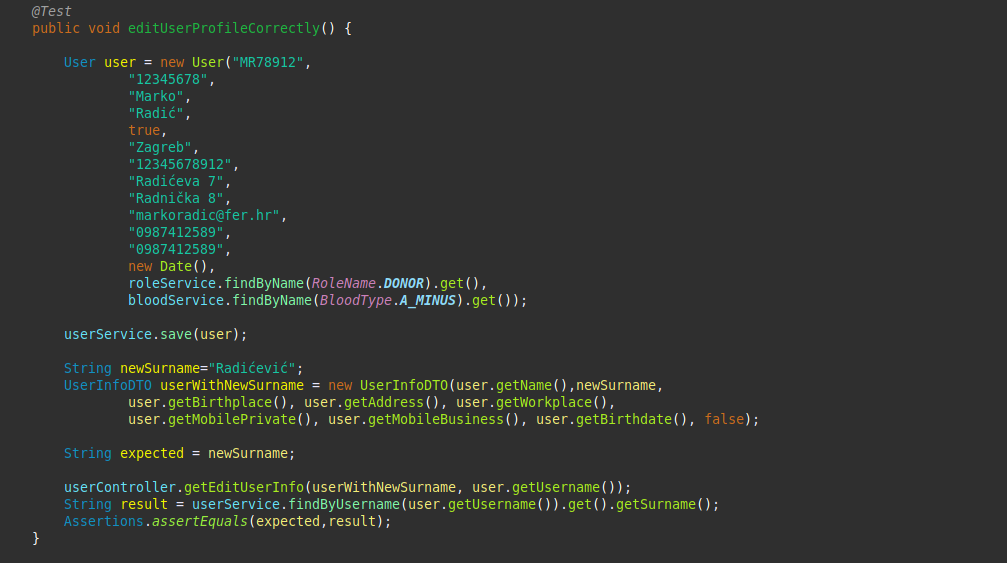
\includegraphics[width=\textwidth, scale=0.5]{slike/unit1}
	\caption{Unit test1}
\end{figure}
{U idućem testu pozivom iste funkcije želimo neuspješno ažurirati polje rejected, koje se ne bi smjelo mijenjati. Na kraju uspoređujemo je li dobivena statusna poruka jednaka očekivanoj "400 BADREQUEST" što bi značilo da aplikacija na pobuđenu situaciju prikladno odgovara.}
\begin{figure}[H]
	\centering
	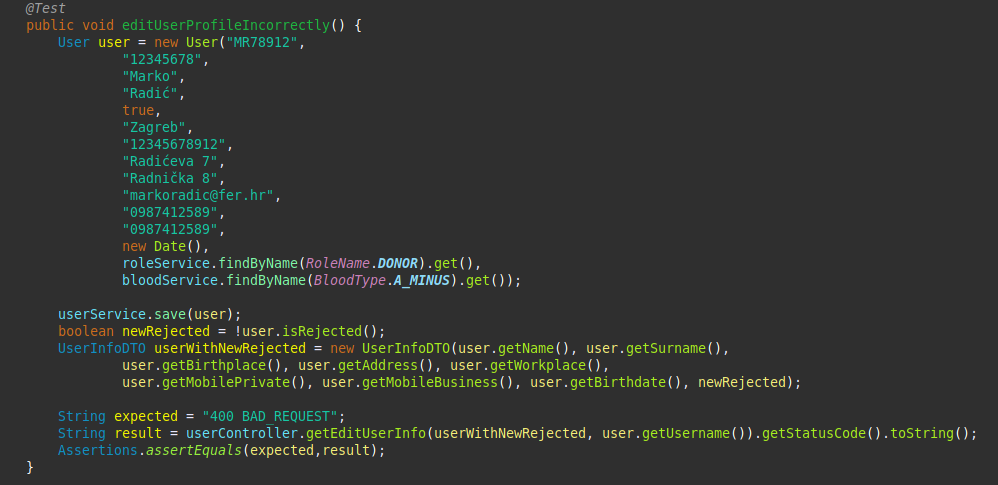
\includegraphics[width=\textwidth, scale=0.5]{slike/unit2}
	\caption{Unit test2}
\end{figure}
\textbf{Promjena optimalnih granica krvi}
\\\\
Pozivom funkcije changeBounds iz klase BloodController želimo uspješno promijeniti donju optimalnu granicu određene krvne grupe. Na kraju uspoređujemo je li donja optimalna granica ažurirane krvne grupe jednaka željenoj granici.
\begin{figure}[H]
	\centering
	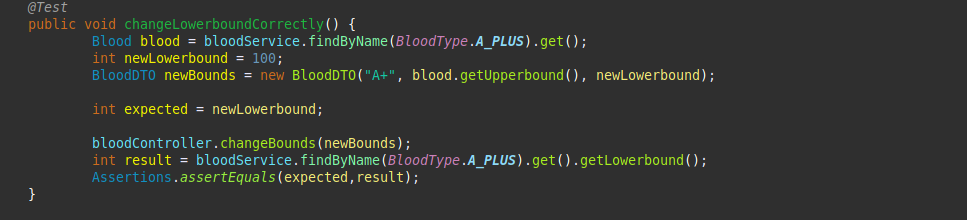
\includegraphics[width=\textwidth, scale=0.5]{slike/unit3}
	\caption{Unit test3}
\end{figure}
\eject
{U idućem testu pozivom iste funkcije želimo neuspješno ažurirati donju optimalnu granicu, koja bi uvijek morala biti pozitivna. Na kraju uspoređujemo je li dobivena statusna poruka jednaka očekivanoj "400 BADREQUEST" što bi značilo da aplikacija na pobuđenu situaciju prikladno odgovara.}
\begin{figure}[H]
	\centering
	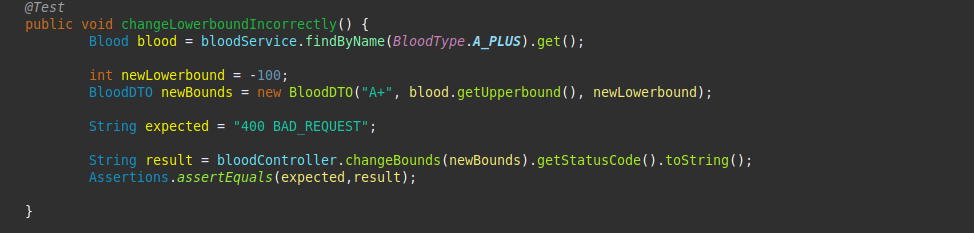
\includegraphics[width=\textwidth, scale=0.5]{slike/unit4}
	\caption{Unit test4}
\end{figure}
\textbf{Evidencija krvi slanjem u instituciju}
\\\\
Pozivom funkcije consumeBlood iz klase ConsumptionController želimo uspješno evidentirati slanje određene krvne grupe u neku instituciju. Na kraju uspoređujemo je li trenutna količina ažurirane krvne grupe jednaka količini umanjenjoj za količinu koja je poslana u instituciju.
\begin{figure}[H]
	\centering
	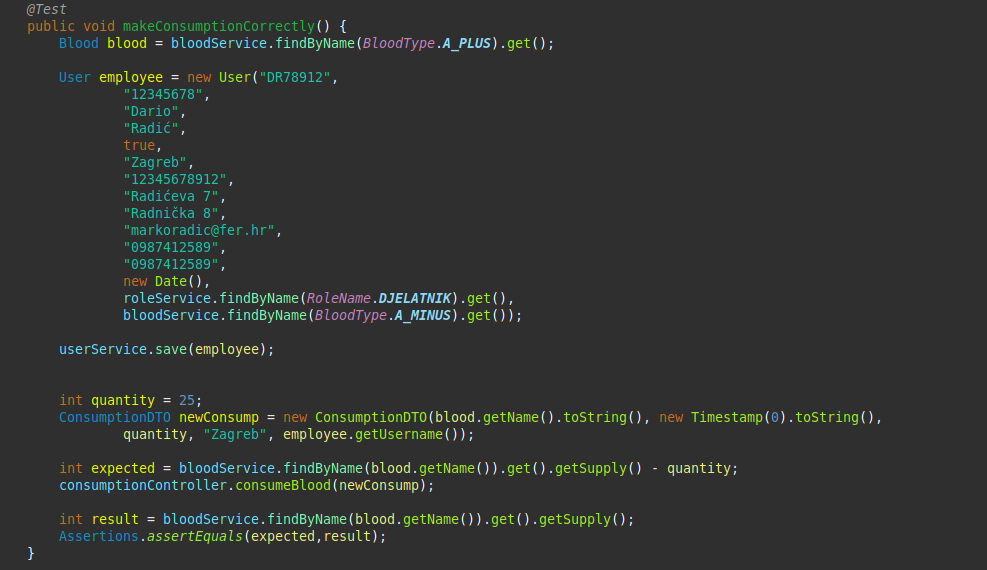
\includegraphics[width=\textwidth, scale=0.5]{slike/unit5}
	\caption{Unit test5}
\end{figure}
\eject	
{U idućem testu pozivom iste funkcije želimo neuspješno evidentirati slanje krvi, čija bi količina uvijek morala biti pozitivna i veća od 0. Na kraju uspoređujemo je li dobivena statusna poruka jednaka očekivanoj "400 BADREQUEST" što bi značilo da aplikacija na pobuđenu situaciju prikladno odgovara. }
\begin{figure}[H]
	\centering
	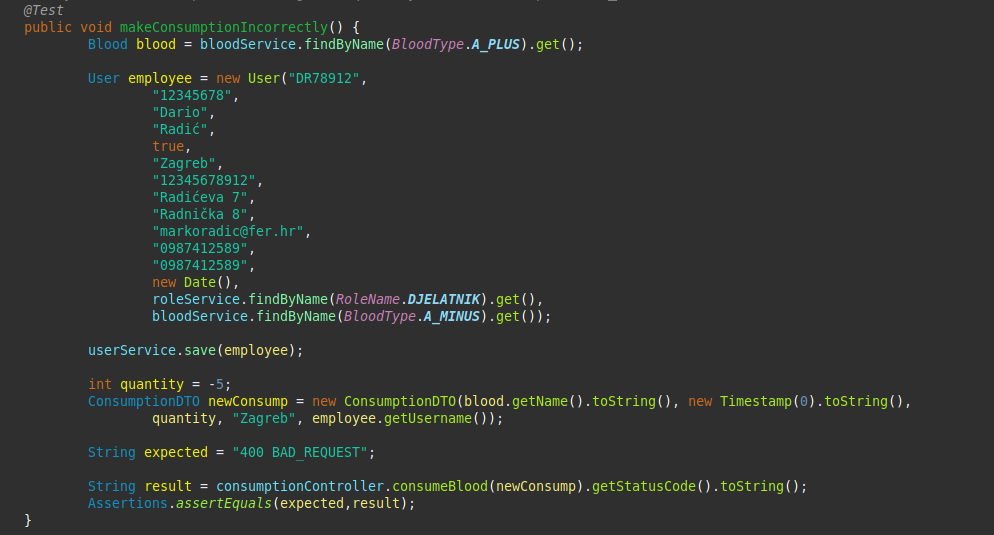
\includegraphics[width=\textwidth, scale=0.5]{slike/unit6}
	\caption{Unit test6}
\end{figure}

\begin{figure}[H]
	\centering
	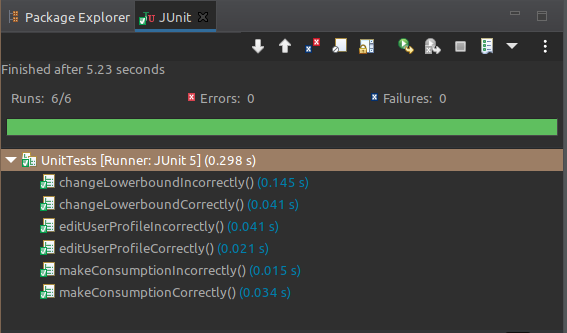
\includegraphics[width=\textwidth, scale=0.5]{slike/unit_testing}
	\caption{Rezultati ispitivanja komponenti}
\end{figure}
\eject
			
			\subsection{Ispitivanje sustava}
			Selenium WebDriver, okvir koji omogućuje programsku interakciju sa internetskim preglednicima, je bio korišten za ispitivanje sustava. Testovi su provedeni na Google Chrome pregledniku. Za sljedeće funkcionalnosti je napravljeno programsko ispitivanje:
			
			 \begin{itemize}
			 	\item {prijava (za donore, djelatnike i admin-a)}
			 	\item {promjene optimalnih granica krvnih grupa (funkcionalnost admin-a)}
			 	\item {evidencija potrošnje krvi (funkcionalnost djelatnika)}
			 	\item {upisivanje donacije u registar (funkcionalnost djelatnika)}
			 	
			 \end{itemize}
		 Korištena je dodatna funkcija za usporavanje sustava, kako se ne bi određeni dijelovi programskog koda za testiranje prerano izvršili:	
\begin{figure}[H]
	\centering
	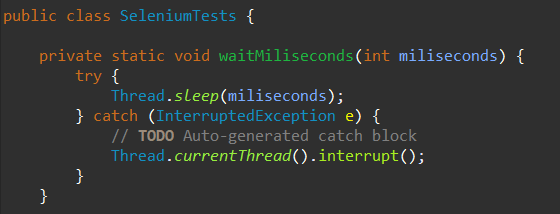
\includegraphics[width=\textwidth, scale=0.5]{slike/wait}
	\caption{Funkcija za usporavanje sustava}
\end{figure}
\eject
\textbf{Prijava}	
\\\\
Ovaj test ima za zadaću ispitati može li se svaka vrsta korisnika sustava ulogirati. Program učitava stranicu i pokušava se ulogirati sa zadanim username­-om i password­-om, te provjera je li doista ulogiran profil za zadani role. Uspjehom se smatra kada je zadani role upisan u drugo polje s desna u gornjoj traci.
\begin{figure}[H]
	\centering
	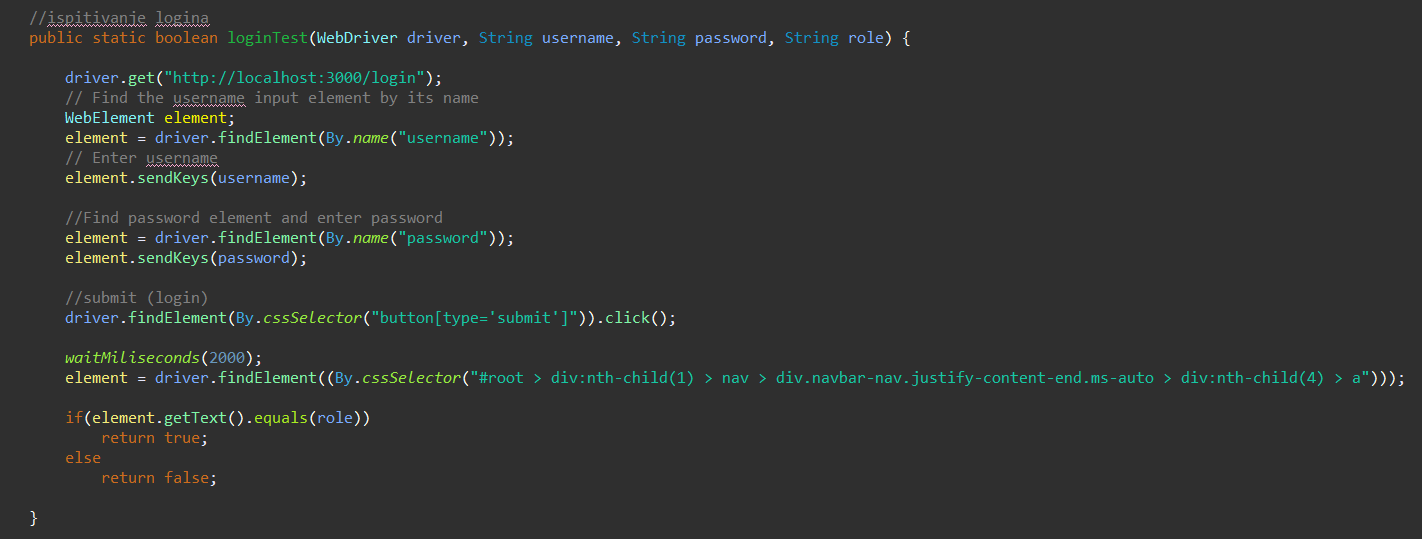
\includegraphics[width=\textwidth, scale=0.5]{slike/selenium1}
	\caption{Selenium test1}
\end{figure}

\textbf{Promjena optimalnih granica krvnih grupa}	
\\\\
Ovaj test ima za zadaću ispitati može li admin postaviti gornju i donju granicu količine krvi određene grupe, koje ako budu pređene dolazi do već spominjanih akcija. Test proglašavamo uspješnim ako poslije pritiska gumba brojevi prikazani u poljima Gornja i Donja odgovaraju željenima.
\eject
\begin{figure}[H]
	\centering
	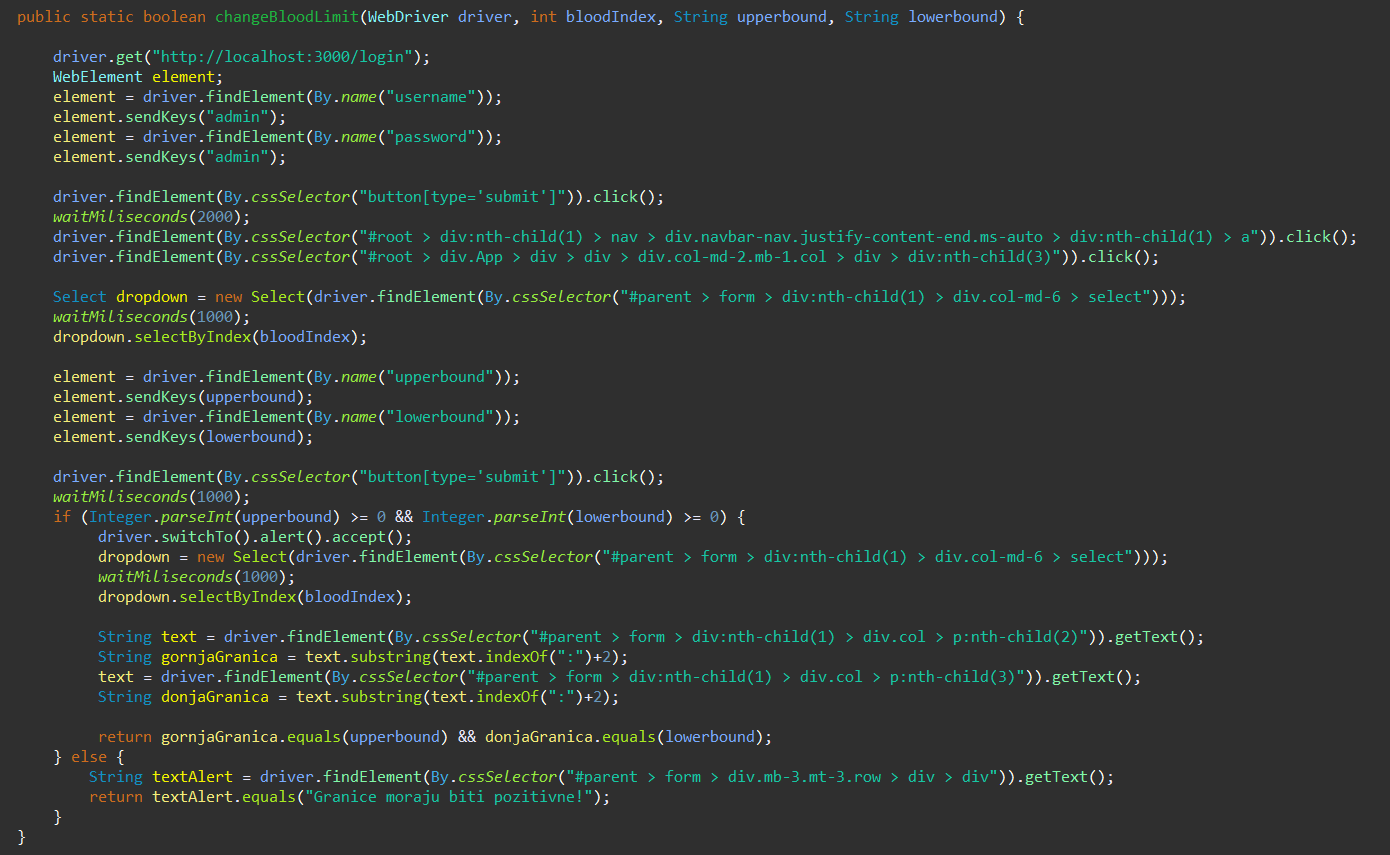
\includegraphics[width=\textwidth, scale=0.5]{slike/selenium2}
	\caption{Selenium test2}
\end{figure}

\textbf{Evidencija potrošnje krvi}	
\\\\
U ovom se testu ispituje može li djelatnik evidentirati slanje krvi u određenu instituciju i odgovara li količina određene krvne grupe u banci nakon slanja očekivanoj količini. Test je uspješan ako je količina krvi određene krvne poslije slanja jednaka očekivanoj. Krv se šalje fiktivnoj lokaciji TESTNA LOKACIJA.
\begin{figure}[H]
	\centering
	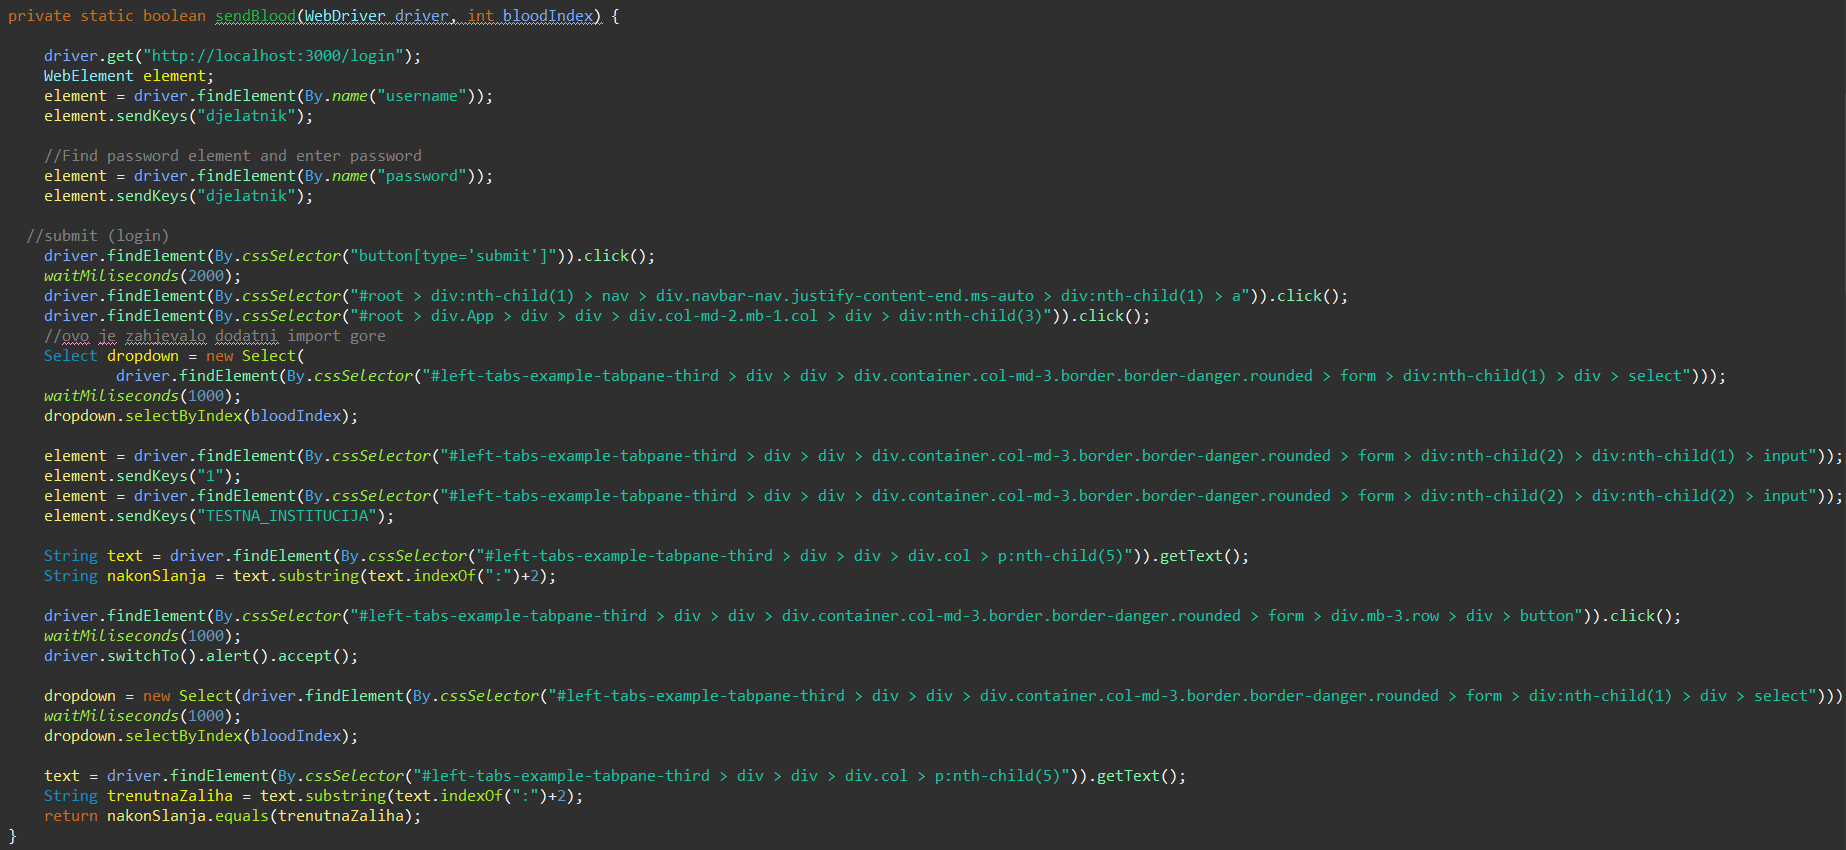
\includegraphics[width=\textwidth, scale=0.5]{slike/selenium3}
	\caption{Selenium test3}
\end{figure}
\eject
\textbf{Upisivanje donacije u registar}	
\\\\
U ovom se testu ispituje može li djelatnik evidentirati obavljenu donaciju (koju je figurativno obavio donor imena TESTDONORNAME na lokaciji TESTLOKACIJA).
Test je prolazan ako preglednik izbaci poruku "Donacija evidentirana" ili "Nije moguće donirati! Nije prošlo dovoljno vremena od zadnje donacije!".
\begin{figure}[H]
	\centering
	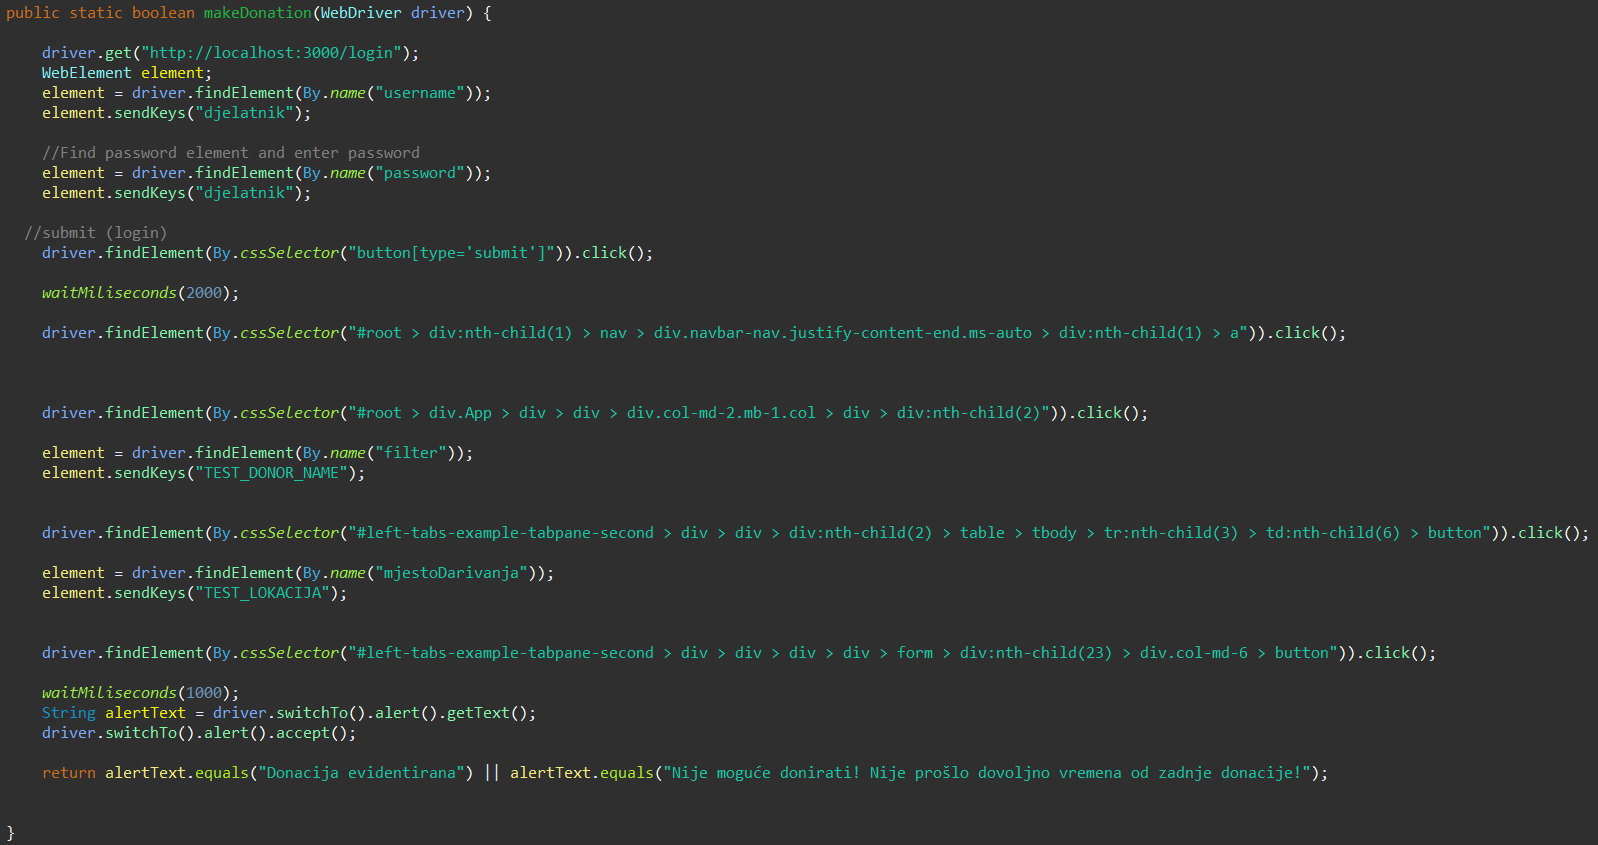
\includegraphics[width=\textwidth, scale=0.5]{slike/selenium4}
	\caption{Selenium test4}
\end{figure}
\eject
Te sve testne funkcije iskoristimo za provođenje testova u glavnoj (main) funkciji:
\begin{figure}[H]
	\centering
	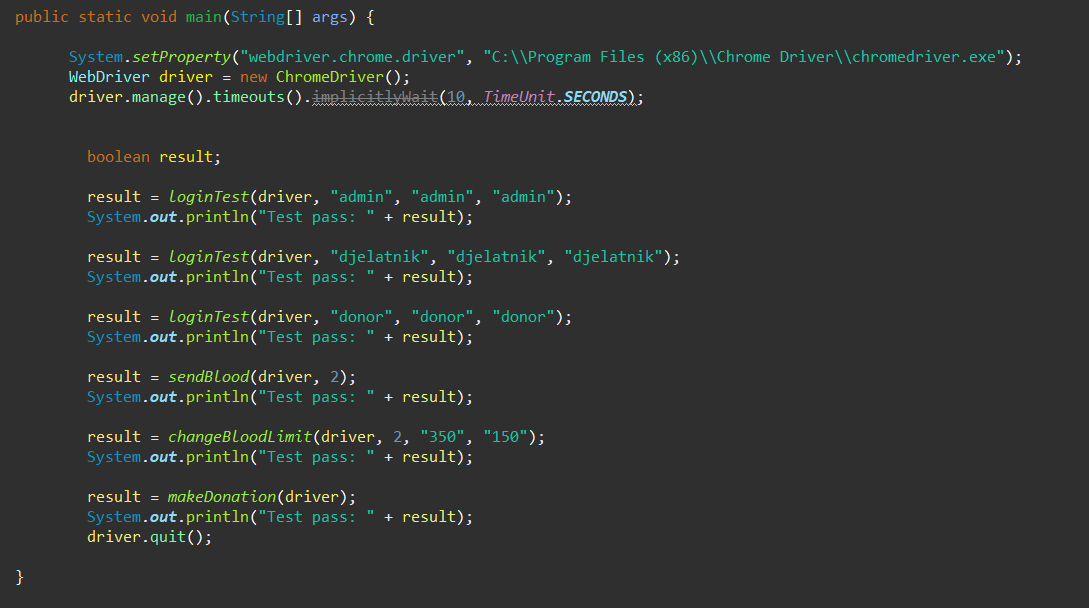
\includegraphics[width=\textwidth, scale=0.5]{slike/main}
	\caption{Funkcija main}
\end{figure}
\begin{figure}[H]
	\centering
	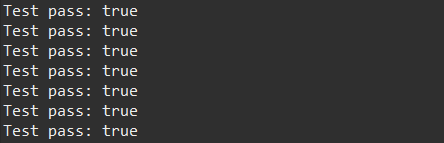
\includegraphics[width=\textwidth, scale=0.5]{slike/rezultat}
	\caption{Rezultat ispitivanja sustava}
\end{figure}
\eject
		\section{Dijagram razmještaja}
			
			Dijagrami razmještaja prikazuju topologiju sustava i odnos sklopovskih i program-
skih dijelova. Olakšavaju nam vizualizaciju razmještaja fizičkog dijela sustava i
sklopovlja. Sustav se sastoji od klijentskog i poslužiteljskog računala. Klijent na
svojem računalu preko web preglednika pristupa aplikaciji. Klijentsko računalo
komunicira s poslužiteljskim računalom preko HTTP veze. Na poslužiteljskom se
računalu nalaze web poslužitelj i poslužitelj baze podataka (PostgreSQL).

\begin{figure}[H]
	\centering
	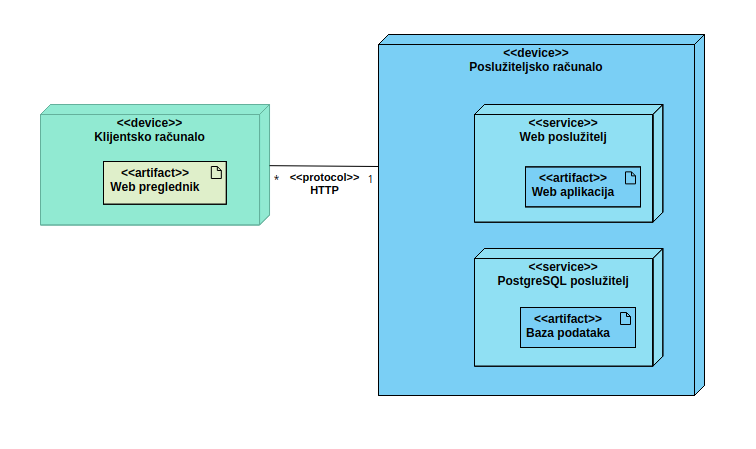
\includegraphics[width=\textwidth, scale=0.5]{dijagrami/dijagram_razmjestaja}
	\caption{Dijagram razmještaja}
	\label{fig:dijagram_razmještaja}
\end{figure}
\eject
	
			
		
		\section{Upute za puštanje u pogon}
		
			\textbf{\textit{dio 2. revizije}}\\
		
			 \textit{U ovom poglavlju potrebno je dati upute za puštanje u pogon (engl. deployment) ostvarene aplikacije. Na primjer, za web aplikacije, opisati postupak kojim se od izvornog kôda dolazi do potpuno postavljene baze podataka i poslužitelja koji odgovara na upite korisnika. Za mobilnu aplikaciju, postupak kojim se aplikacija izgradi, te postavi na neku od trgovina. Za stolnu (engl. desktop) aplikaciju, postupak kojim se aplikacija instalira na računalo. Ukoliko mobilne i stolne aplikacije komuniciraju s poslužiteljem i/ili bazom podataka, opisati i postupak njihovog postavljanja. Pri izradi uputa preporučuje se \textbf{naglasiti korake instalacije uporabom natuknica} te koristiti što je više moguće \textbf{slike ekrana} (engl. screenshots) kako bi upute bile jasne i jednostavne za slijediti.}
			
			
			 \textit{Dovršenu aplikaciju potrebno je pokrenuti na javno dostupnom poslužitelju. Studentima se preporuča korištenje neke od sljedećih besplatnih usluga: \href{https://aws.amazon.com/}{Amazon AWS}, \href{https://azure.microsoft.com/en-us/}{Microsoft Azure} ili \href{https://www.heroku.com/}{Heroku}. Mobilne aplikacije trebaju biti objavljene na F-Droid, Google Play ili Amazon App trgovini.}
			
			
			\eject 